\documentclass[runningheads,a4paper]{llncs} \usepackage[utf8]{inputenc}
\usepackage[hyphens]{url}
\usepackage{graphicx}
\usepackage{hyperref}
\usepackage{float}
\usepackage{eurosym}
\usepackage[normalem]{ulem}
\usepackage{alltt}
\usepackage{amssymb}
\usepackage{listings}
\usepackage{subfigure}
\setcounter{tocdepth}{3}

\usepackage{url}
\newcommand{\keywords}[1]{\par\addvspace\baselineskip
\noindent\keywordname\enspace\ignorespaces#1}

\begin{document}

\mainmatter  % start of an individual contribution

% first the title is needed
\title{Context-aware Querying for\\ Multimodal Search Engines}

% a short form should be given in case it is too long for the running head
\titlerunning{Context-aware Querying for Multimodal Search Engines}

\author{Jonas Etzold\inst{1} \and Arnaud Brousseau\inst{2} \and Paul Grimm\inst{1} \and Thomas Steiner\inst{2}}

\authorrunning{Context-aware Querying for Multimodal Search Engines}
% (feature abused for this document to repeat the title also on left hand pages)

% the affiliations are given next; don't give your e-mail address unless you
% accept that it will be published
\institute{Erfurt University of Applied Sciences, Germany, \email{\{jonas.etzold|grimm\}@fh-erfurt.de}
\and Google Germany GmbH, ABC-Str. 19, 20354 Hamburg, Germany,
\email{\{arnaudb|tomac\}@google.com}}

\maketitle

\begin{abstract}
Multimodal interaction provides the user with multiple modes of interacting with
a system, such as gestures, speech, text, video, audio, etc. A multimodal system allows for several distinct means for input and output of data. In this paper, we present our work in the context of the \mbox{I-SEARCH} project, which aims at enabling context-aware querying of a multimodal search framework including real-world data such as user location or temperature.

% @TOMAC by PG: Etwas mehr Inhalt als "present our work in the context of.." 
% f�nde ich gut: z.B. Nennung der Konzept MMBag, ... sowie recommendations 
% der User Study

\keywords{Multimodality, Context Awareness, User Interfaces}
\end{abstract}

\section{Introduction}
The \mbox{I-SEARCH} project aims to provide a unified framework for multimodal content indexing, sharing, search and retrieval. This framework will be able to handle specific types of multimedia and multimodal content, namely text, 2D images, hand-drawn sketches, videos, 3D objects and audio files), but also real world information that can be used as part of queries. Query results can include any available relevant content of any of the aforementioned types. This is achieved through Rich Unified Content Annotation (RUCoD), a concept that we have introduced in~\cite{ijmis}. It becomes clear that a framework like \mbox{I-SEARCH} faces specific challenges user interface-wise. Not only does it have to allow for the combination of multimodal queries, but it has to do so on different devices, both desktop and mobile. This research being conducted in the context of a European research project, we have time constraints to take into account, hence, we can time-wise simply not afford to develop two UI stacks separately for desktop and mobile. We show how using newly added features in the markup language HTML  we can kill these two flies with one stone.

The remainder of this paper is structured as follows: Section~2 presents related work, Section~3 introduces our chosen methodology, split up in three sub-tasks, Section~4 goes into implementation details and presents some preliminary results, Section~5 presents an Evaluation of a user study that we have conducted, Section~6 ends the paper with an outlook on future work and provides a conclusion.

\section{Related Work}
\label{sec:related}

% @JE by PG: eher "to improve" statt "better" im n�chsten Satz

Many people have been involved in the research of better user
interfaces (UI) for search tasks in the last few years. They widley found
evidence for the importance and special demand on the design of search user
interfaces in order to achieve an effective and useable search \cite{hearst2009}
\cite{quesenbery2008} \cite{huangTsaiChang2009}. Especially with the emerging
of Web 2.0 and the vast amount of user generated content, the raise of the big
search engines, like Google and Bing continued and search became one of the
main tasks in our daily internet usage \cite{quesenbergWeb2008}. This trend
further increases the importance of the interaction with and the design of
search engines and also raises the need for extending search tasks
beyond textual-queries on desktop system. In this manner Hearst
\cite{hearst2011} describes emerging trends for search interface design, which
include that interfaces have to be more device-independent (i.e. for mobile
devices) and be able to support the creation of multimodal search
queries where text can be enriched with multimedia and real-world data in order
to deliver more precise results. 

With the development of multimodal search interfaces also concepts for
multimodal interaction, like defined by Nigay et al. \cite{nigay} become a
important aspect to distribute all features of this new type of search
interfaces to the user. Rigas \cite{rigas2007} also found evidence that the use
of multimodal features of a search interface, e.g. speech or graphs can support
the usability of the whole search engine. 
In order to combine the efforts towards multimodal interaction the W3C follows
an approach to create an framework which is described by the W3C Multimodal
Interaction Working Group with its work-in-progress specification of the
``Multimodal Architecture and Interfaces'' \cite{w3cMMI}. Hereby the framework
is used to describe the internal structure of a certain interaction component,
including the in- and outputs of the various interaction types based on XML.
Serrano et al. further created the OpenInterface Framework \cite{openinterface},
which allows to flexible create combined interaction pipelines which use several
input channels (e.g. speech and touch). Other approaches to provide frameworks
for multimodal interaction and interfaces are described by Sreekanth
\cite{sreekanth}, who uses a Monitor Agent to collect events from different
modalities and Roscher \cite{roscher}, who uses the Multi-Access Service
Platform (MASP) which implements different user interface models for each input
modality and is able to combine them to more complex multimodal user interfaces
including the synchronization of all inputs along the user interface models.

The possibilty to generate more complex but also more effective search queries
with multimodal search interfaces as well as the nature of the internet as an
enviroment where people can assist each other make the integration of
collaborative interaction approaches for search engines interesting. Mainly the
work of Morris \cite{morris2007} and Pickens \cite{pickens2008} described
interesting ways of collaborative search approaches. They make use of a search
session and state variables in user profiles to transfers changes made in the
interface of one user to all other collaborating users and vice versa. Further
the survey about collaborative web search practices done by Morris
\cite{morris2008} as well as the status quo practices presented by Amershi
\cite{amershi2009} proof the need and practicability of collaborative search
methods.

\section{Methodology}
In this Section we present our methodology for context-aware querying for multimodal search engines, split up in three sub-tasks \emph{MMBag}, \emph{UIIFace}, and \emph{CoFind}.

% @JE by PG: mit den K�rzeln kann kein Leser etwas anfangen -->
% eher beschreibend auff�hren

% by PG: instead of MMBag use a more desribing title like: 
% Interface for combining different search modalities
% (same problem with next subtitles )

\subsection{MMBag}
MMBag stands for Multi-Modal Bag and designates the \mbox{I-SEARCH} User
Interface. It comes with specific requirements linked with the need for users to use multiple types of input: audio files or stream, video files, 3D objects, hand drawings, real-world information such as geolocation or time, image files and of course, plain text. This part of the paper shows the approach chosen to create MMBag.

Multimodal search engines are still very experimental at the time of writing. When building MMBag, we tried to look for a common pattern in search-related actions. Indeed, MMBag remains a search interface at its core. In order for users to interact efficiently with \mbox{I-SEARCH}, we needed a well-known interface paradigm. Accross the Web, a pattern has the monopoly for search related actions:  the text field, where a user can focus, enter her query, and trigger subsequent search actions. From big Web search engines such as Google, Yahoo or Bing, to small internal search engines, the pattern stays the same. 

However, \mbox{I-SEARCH} can't directly benefit from this broadly accepted pattern, as a multimodal search engine must accept a large number of types of input at the same time: audio, video, 3D objects, sketches, etc. How can this be achieved? Some search engines, even if they don't have the need for true multimodal querying, do have the need to accept input which is not plain text.

As a first example, we consider TinEye\footnote{\url{http://www.tineye.com/}}. TinEye is a Web-based search engine that allows for query by image content (QBIC) in order to retrieve similar or related images. The interface is split in two distinct parts: one part is a text box to provide a link to a Web-hosted image, while the second part allows for direct file upload (Figure~\ref{fig:tineye-ui}). This interface is a good solution for a search engine like TinEye (image input, image output) but \mbox{I-SEARCH} will need to come with more options than that.
\begin{figure}[h!]
  \centering
    
\includegraphics[width=0.8\linewidth]{resources/tineye-UI.png}
  \caption{Extract from the TinEye User Interface}
  \label{fig:tineye-ui}
\end{figure}

As a second example, we examine MMRetrieval\footnote{\url{http://www.mmretrieval.net}}~\cite{mmretrieval}. It is an attempt at bringing together image and text search to compose a multimodal query. MMRetrieval is a good showcase for the problem of designing a user interface (UI) with many user-tweakable options. For a user from outside the Information Retrieval field, the UI seems not necessarily clear in all detail, especially when specific terms such as \emph{Image ARF} are used (Figure~\ref{fig:mmretrieval-ui}).

\begin{figure}[h!]
  \centering
    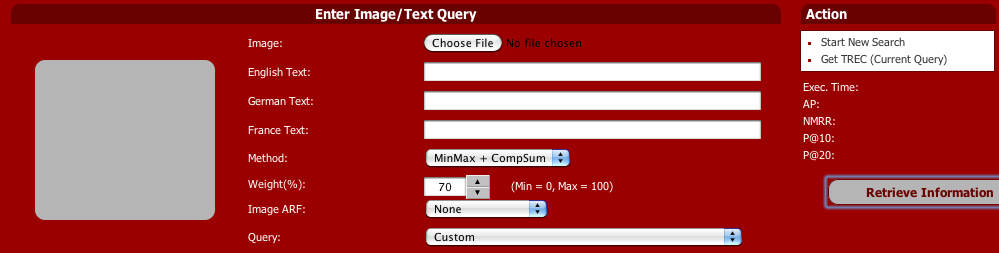
\includegraphics[width=0.8\linewidth]{resources/mmretrieval-UI.png}
  \caption{Extract from the MMRetrieval User Interface}
  \label{fig:mmretrieval-ui}
\end{figure}

Finally, we have a look at Google Search-by-image, a functionality launched on June, 14, 2011\footnote{\url{http://googleblog.blogspot.com/2011/06/knocking-down-barriers-to-knowledge.html}} and has the same requirements as MMRetrieval in terms of user interface, i.e., combining text and image input. With the Search-by-image interface, Google has succeeded in keeping the text box pattern (Figure~\ref{fig:search-by-image-box}), while preventing any extra visual noise. The interface is \emph{progressively disclosed} to users via a contextual menu when the camera icon is clicked (Figure~\ref{fig:search-by-image-popup}).

\begin{figure}[h!]
  \centering
    
\includegraphics[width=0.8\linewidth]{resources/search-by-image-UI-box.png}
  \caption{Input for the Search-by-image UI}
  \label{fig:search-by-image-box}
\end{figure}

\begin{figure}[h!]
  \centering
    
\includegraphics[width=0.8\linewidth]{resources/search-by-image-UI-popup.png}
  \caption{Popup for the Search-by-image UI}
  \label{fig:search-by-image-popup}
\end{figure}

Even if the Search-by-image solution seems very elegant, this is still not suitable for \mbox{I-SEARCH} since the interface would require a high number of small icons: camera, 3D, geolocation, audio, video, etc.  As a result, we decided to adapt a solution that can be seen in Figure~\ref{fig:isearch-ui}. This interface keeps the idea of a single text box. It is enriched by auto-completion as well as ``tokenization". The term ``tokenization" refers to the process of representing an item (picture, sound, etc.) with a small token in the text field, as if it was part of the text query. We also kept the idea of progressive disclosure for the different actions required by the various modes, e.g., uploading a picture or sketching something. The different icons are grouped together in a separated menu, close to the main search field.

\begin{figure}[h!]
  \centering
    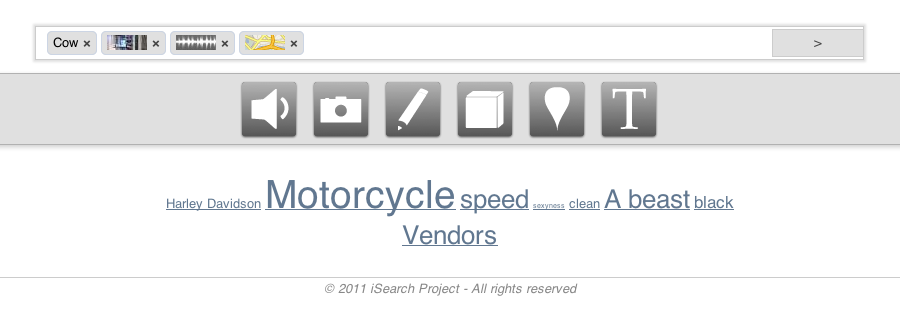
\includegraphics[width=0.8\linewidth]{resources/isearch-UI.png}
  \caption{First version of \mbox{I-SEARCH} interface}
  \label{fig:isearch-ui}
\end{figure}

\subsection{UIIFace}

Interaction is an important factor when it comes to context-awareness and
multimodality. In order to deliver a Graphical User Interface (GUI) which is
able to facilitate all the possibilities of an multimodal search engine, an
very flexible approach with a rich interaction methodology is needed. 
Further multimodal quering could also involve the way a user interacts with the
system as part of the query. 

To target all those needs the concept of UIIFace (Unified Interaction Interface)
is introduced as general interaction layer for context-arwe multimodal quering.

UIIFace describes a common interface between these interaction modalities and the 
graphical user interface (GUI) of \mbox{I-SEARCH} by providing a general set of interaction 
commands for the interface. Each input modality provides the implementation 
for parts of the commands or all commands defined by UIIFace. 

The idea of UIIFace is based on the OpenInterface Framework \cite{openinterface}
which describes a framework for the development of multimodal input interface
prototypes. It uses components which can represent different input modalities as
well as user interfaces and other required software pieces in order to create
and control a certain application. In contrast to this approach UIIFace is a web
implemented approach based on modern HTML5 libraries. Furthermore it provides a
command interface to web based GUIs instead of being able to create a
stand-alone application outside the browser window.

For creating the set of uni- and multimodal commands which can be used for
\mbox{I-SEARCH} interfaces, the results of Chang \cite{chang} as well as the needs
derived from the creation of multimodal search queries are used.

\begin{figure}[h!]
  \centering
    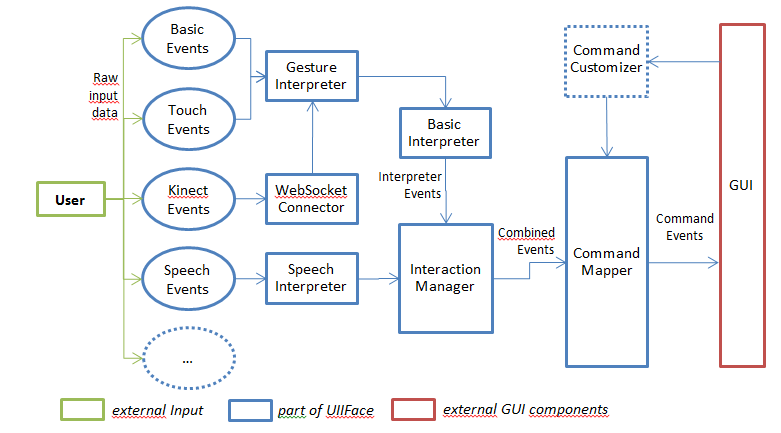
\includegraphics[width=0.8\linewidth]{resources/uiiface-structure.png}
  \caption{Schematic view on the internal structure of UIIFace}
  \label{fig:uiiface}
\end{figure}

Figure \ref{fig:uiiface} depicts the internal structure of UIIFace and shows the
flow of events. Events are raised from the users raw input. Gesture Interpreter
determines defined gestures (e.g. zoom, rotate) found in the raw input. If no
gestures were found, the Basic Interpreter routes Touch and Kinect events to
basic cursor and keyboard events. Gestures, speech commands and basic mouse,
keyboard events are then synchronized in the Interaction Manager and forwarded
as Combined Events to the Command Mapper which maps the incoming events to the
defined list of interaction commands which can be registered by any web-based
GUI. The Command Customizer can be used to rewrite the trigger event for
commands to user specific gestures or other input sequences (e.g. Keyboard
shortcuts). This is an additional feature which is not crucial to the
functionality of UIIFace but can be implemented at a later stage in order to add
more explicit personalisation features.

In contrast to the approaches mentioned in chapter \ref{sec:related}
UIIFace does not deliver any UI components and will remove the need for an
interface developer to take care of the input modality through the unified
command layer which provides practically modality-independent interaction
commands.

\subsection{CoFind}

Another part of our methodology targets the increased complexity of search
tasks and the necessity to collaborate on those tasks in order to formulate
adequat search queries which lead faster to appropriate result. The increased
complexity is primarly caused through the vast amount of unstructured data 
within the Internet and secondly through situations where the expected results
are very fuzzy or hard to describe in textual terms. 

Therefore the CoFind (Collaborative Finding) approach is introduced as an
collaborative search system which enables real-time collaborative search query
creation on a pure html website.

Likewise the collaborative approach of Google Tables and Documents the
system enables people and expert users from different domains to work together.
The main difference here is that CoFind enhances the idea of collaborative document
creation to search queries. This extension becomes even more important if
search engines allow the usage of multimodal search queries which
involve multimedia, real-world and user data in a query. 

The CoFind concept is based upon a search session concept in which HTML content
of the participants local clients is transmitted within this session.
In order to realise collaborative querying the concept provides functions for
activating collaborative search sessions, joining other online users by their
Email address and managing messaging between participants of the search session.

In general the concept consists of three main parts:
\begin{enumerate}
  \item Session Manager - controls establishment and closing of collaborative
  search sessions
  \item Content Manager - transmission of changes in user interfaces to all
  participants
  \item Messaging Manager - transmission of status and user messages to all
  participants
\end{enumerate}

Figure \ref{fig:cofind} shows how the parts of the Collaborative Search concept
interact during the search process in order to create a collaborative search session.

\begin{figure}[h!]
  \centering
    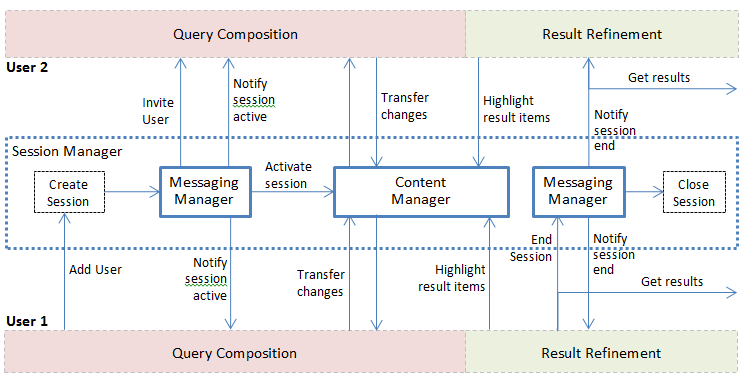
\includegraphics[width=0.8\linewidth]{resources/cofind-workflow.png}
  \caption{Schematic diagram of interaction between parts of CoFind}
  \label{fig:cofind}
\end{figure}
 
The main flow of a collaborative search session can be described as follows:
\begin{enumerate}
  \item To create or join a collaborative search session a user must supply the
  email address of the other user
  \item If the other user is online and logged-in he receives an on-screen
  message and needs to accept the joining of the other user
  \item after confirmation a new session entry is created which stores all
  participants
  \item every time a change on the query input field or result set is performed,
  the changed content is transferred to all participants 
  \item each participant is able to search and navigate through the result set
  independent from others, but selected results can be added to collaborative
  result set
  \item the search session is closed after all users left the session
  or logged out from the system
\end{enumerate}

The advantages of the described concept are:
\begin{enumerate}
  \item allows collaboration on query compilation across multiple devices and
  users
  \item no interface overhead, easy to create collaborative sessions
  \item allows more precise query formulation for difficult search tasks
\end{enumerate}

\section{Implementation and Results}

The \mbox{I-SEARCH} GUI is built using the Web platform. HTML, CSS and
JavaScript are the three main building blocks for the interface. The rationale
behind that choice is the following: \mbox{I-SEARCH} needs to be cross-browser
and cross-device compatible. The latest specifications of those technologies
enable us to do just that. Indeed, CSS3~\cite{css3}, HTML5~\cite{html5} and the
therein defined new JavaScript APIs empower the browser in truly novel ways.

Our strategy also includes support for older browsers. When browsing the Web, a
significant part of users don't have access to a cutting-edge Web browser. If a
feature we use is not available for a certain browser version, two choices are
available: either drop support for that feature if it is not important (e.g.,
drop visual shims like CSS shadows or border-radius), or provide alternate
solution to mimic the experience.

We would like to highlight that CSS and HTML are 2 standards that natively
enable progressive enhancement thanks to a simple rule: when a Web browser
doesn't understand an HTML attribute, a CSS value or selector, it simply
\emph{ignores it}. This rule is the guarantee that we can build future-proof
pages using CSS and HTML. Web browsers will render the page according to their
capabilities: old browsers will render basic markup and styles, while modern
browsers will be able to render stunning CSS3 effects.

Of course, progressive enhancement isn't always a good solution, particularly
when you want to ensure that all users can access a particular feature. In this
case, we will use the \emph{graceful degradation} principle, i.e, we will use
fallback solutions when the technology stack is not there to support our needs
in a certain browser.

The next parts of this paper discuss, in the case of \mbox{I-SEARCH}, why the
use of certain features make sense, and how we plan to use them. We will look at
semantic markup, media-queries, canvas, audio and video, geolocation, sensors
integration, and device API.

\subsection{HTML5 Semantic Markup} 

HTML5 comes with extra elements to add meaning to Web pages, such as {\tt <header>}, {\tt <footer>}, {\tt <nav>} or {\tt <time>}, to name a few\footnote{The complete set of elements introduced in HTML5 can be found at \url{http://dev.w3.org/html5/spec/Overview.html\#semantics}}. It makes sense in the case of \mbox{I-SEARCH} to use more semantic markup: it will greatly improve usability and interoperability\cite{}.
The lack of support in older browsers in not a problem here: extra semantic simply won't be provided.

\subsection{CSS3 Media Queries} 

The \mbox{I-SEARCH} project needs to be compatible with a large range of devices: desktop browsers, phones and tablets. Rather than building several versions of \mbox{I-SEARCH}, we will use CSS3 Media-queries\footnote{\url{http://www.w3.org/TR/css3-mediaqueries/}} to adapt the layout to those devices. Media-queries are not supported in old browsers such as Internet Explorer (version prior to 8) or Mozilla Firefox (version prior to 3.5), but that is not an issue since tablets and phones have browsers that support this feature.

To show our exact strategy, here is how and where different devices are supported by the combination of normal CSS selectors and CSS Media-Queries: 
\begin{itemize}
\item Begin the styling with a global CSS reset, so that styles are consistent across browsers. It gives a common basis.
\item Then come the global styles, suitable for old and modern browsers.
\item Finally, we can add CSS3 enhancements, including Media-Queries. This will be ignored by old browsers, but as pointed earlier, it is not an issue.
\end{itemize}

\subsection{Canvas}

Canvas in HTML5 refers to the introduction of a new element: {\tt <canvas>}\footnote{\url{http://www.whatwg.org/specs/web-apps/current-work/multipage/the-canvas-element.html}}. This element enable cheap and scriptable rendering of graphics. For instance, since the introduction of {\tt <canvas>} in modern browsers, many HTML5 games have been written because {\tt <canvas>} offers a convenient and fast way to deal with user input and graphic rendering in real-time through its Javascript API. 

In the case of \mbox{I-SEARCH}, our plan is to use {\tt <canvas>} for user input when the query requires a user sketch, and also to display results in novel ways. Indeed, {\tt <canvas>} enables virtually any kind of result visualization, including visualization of audio and video.

{\tt <canvas>} will be a core element of \mbox{I-SEARCH}. Thus, it is crucial to offer a fallback option for older browsers. We plan to do so by using FlashCanvas\footnote{\url{http://flashcanvas.net/}}.


\subsection{HTML5 Audio and video}
HTML5 comes with 2 new elements, {\tt <audio>} and {\tt <video>}, to deal with multimedia elements. The key difference is that video and audio items are now fully rendered in the browser. It means that audio and video are now fully scriptable: rotation, scale, controls, CSS Styles, and so forth. 

In the case of \mbox{I-SEARCH}, this flexibility brought by HTML5 {\tt <audio>} and {\tt <video>} is a huge opportunity to create interesting and interactive visualisations of search results.
If  {\tt <audio>} and {\tt <video>} are not available in a certain browser, we will use Adobe Flash\footnote{\url{http://www.adobe.com/products/flashplayer/}} to display media items to users.

\subsection{File API}

The file API is a Javascript API, part of the HTML5 Specification. It ``provides an API for representing file objects in web applications, as well as programmatically selecting them and accessing their data."\footnote{\url{http://www.w3.org/TR/FileAPI/}}. 

This is particularly interesting in the case of \mbox{I-SEARCH}, since users are very likely to compose their query with local files (piece of music, pictures from their local library, etc). The File API allows new paradigm to deal with files, such as native support for drag'n'dropping elements from the desktop to the \mbox{I-SEARCH} interface.

This feature is not crucial for user interaction, so we won't provide fallback for older browsers. Indeed, a simple form with the possibility to upload a file will be provided, as shown in figure \ref{fig:input-picture}.
 
\begin{figure}[h!]
  \centering
    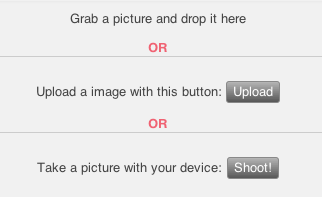
\includegraphics[width=0.3\linewidth]{resources/input-picture.png}
  \caption{Picture panel of the \mbox{I-SEARCH} interface}
  \label{fig:input-picture}
\end{figure}

\subsection{Geolocation}
Context-aware search is one of the features of the \mbox{I-SEARCH} framework.
This is particularly useful in the case of a user searching on a mobile device.
Indeed, he/she is more likely to need information relative to his/her location.

HTML5 comes with a Javascript API that does just that: the geolocation API.
Instead of checking the IP address and/or calling the GPS of a device through
proprietary API, the geolocation API enables Web pages to retrieve a user's
location with only one line of Javascript:
\begin{lstlisting}
navigator.geolocation.getCurrentPosition()
\end{lstlisting}
In the background, the browser calls the device GPS or compute an approximate
location thanks to IP address information. Furthermore, the retrieval of a
user's location is much more transparent since browsers supporting the
geolocation API prompt users for their permission before doing anything. See
figure \ref{fig:geolocation-prompt}.

\begin{figure}[h!]
  \centering
    
\includegraphics[width=0.3\linewidth]{resources/geolocation-prompt.png}
  \caption{Firefox 5, asking permission to share user location}
  \label{fig:geolocation-prompt}
\end{figure}


\subsection{Sensors}

Another aspect which is important for context-awareness is the use of
hardware sensors integrated or attached to different device types. 
Knowing the orientation and acceleration of a device or capturing the user
in 3D space in order to detect gestures or
Mainly in mobile devices accelerometers and gyroscopes are integrated and
can be accessed through the device specific APIs. 

HTML5 comes with specific events that target those sensors and define unified
events bundeled together in the specification for the \emph{DeviceOrientation}
Event \cite{deviceOrientation}. Referring the specification the orientation of
the device can be retrieved with the following Javascript code:
\begin{lstlisting}
window.addEventListener('deviceorientation', function(event) {
  var a = event.alpha;
  var b = event.beta;
  var g = event.gamma;
}, false);
\end{lstlisting}

Other attached sensors like a depth-sensor for tracking people in 3D space
does not have a standard with which their data can be captured in a browser
enviroment. For those sensors we create tiny service applications which capture
the sensor data and stream that with the help of HTML5 websockets
\cite{websockets} to any browser.

\subsection{Device API}



\section{Evaluation}

To validate our interface design on tasks of multimodal search we conducted a
user study. We used a comparative study design to explore how the usage of
different media types should look like and how these can influence the success
rate of search queries. Overall, we expected that the user can handle the user
interface easily and he gets a result which satisfies his needs. We therefore
set the following hypothesis: (H1) a user will start a search query with just one media type, (H2) search refinement will be done by adding other media types
or removing them, (H3) all media types are handled similarly.

%\begin{enumerate}
%  \item (H1) a user will start a search query with just
%one media type,
%  \item (H2) search refinement will be done by adding other media types
%or removing them,
%  \item (H3) all media types are handled similarly. 
%\end{enumerate}

For the user study we recruited seven participants (six male and one female)
aged between 20 and 35. All participants were familiar with textual web-based
search. We asked all study participants to find three different items (sound of
a tiger, one 3D model of a flower and one image of a car, see Figure ABCD). For
explanation, what should be retrieved, these items were shown in their original
format to the study participants. To perform the search queries a mobile
notebook with touch display was used. Our goal was to validate our interface
design as well as to measure the impact of the possibility of multimodal search. 

\begin{figure}[h!]
\subfigure[Sound of a tiger]{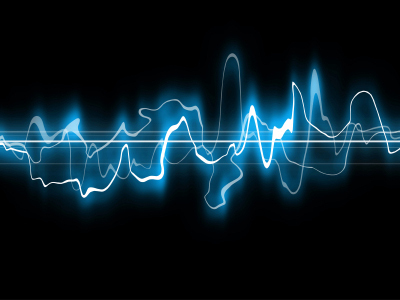
\includegraphics[width=0.3\textwidth]{resources/sound-tiger.jpg}}\hfill 
\subfigure[3D model of a flower]{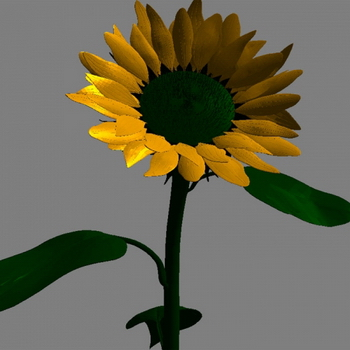
\includegraphics[width=0.3\textwidth]{resources/3d-flower.jpg}}\hfill 
\subfigure[Image of a car]{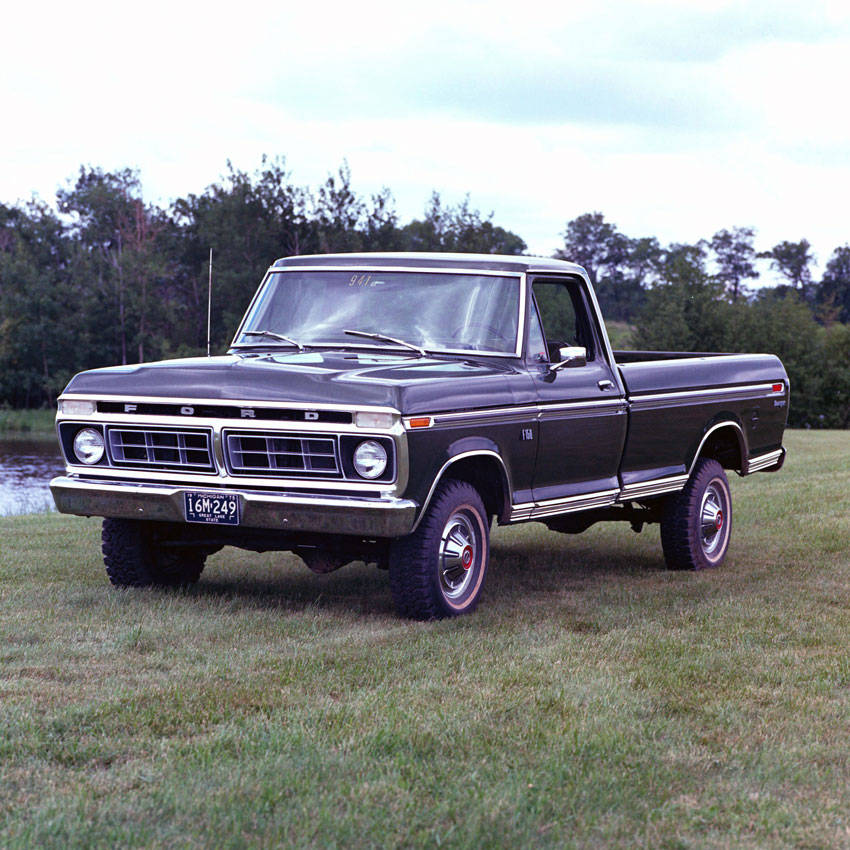
\includegraphics[width=0.3\textwidth]{resources/image-pickup.jpg}}
\caption{Sample search items used for user study}
\end{figure}

In general, we observed that the concept of multimodal search was new and
unfamiliar to all participants. Before the user study, for all participants a
web-based search and a text-based search have been identically. Using I-Search
they have to become aware of the possibility of the meaning of different media
types and of multimodal interaction (see Table ABCD). Our hypothesis (H1) is not
supported statistically. It depends highly on the behavior of each individual
person whether one or more search item or media type is used. In combination
with (H2) a conclusion out of the interviews is, that adding search items as
well as customizing them has to be as easy as possible. The participants do not
suffer obstacles in using one special media type. Thus, if one media type is
difficult to use, they avoid using it by using different media types, also if
this implies, that the search query will be more complicated and challenging.
This applies also to hypothesis (H3). In order to allow multimodal search
queries, the following recommendations can be derived from the user study: 

\begin{enumerate}
  \item No media type should be privileged
  \item The handling of all media types should be as similar as possible
  \item Search refinement should be possible in result presentation  
\end{enumerate}

\section{Conclusion and Future Work}
(Tom)

\section{Acknowledgments}
This work is partly funded by the EU FP7 \mbox{I-SEARCH} project under project reference 248296.

\bibliographystyle{plain}
\bibliography{mmm2012}
\end{document}
